\chapter{Security at the physical layer}
As already mentioned in section \ref{sec:intro}, the wireless channel has no inherent security mechanisms. 
As a result, The wireless communication medium is open to \textbf{jamming} (or interference) and 
\textbf{eavesdropping} attacks from intruders.\\
Furthermore, the attacks can be classified into two categories: 
\begin{itemize}
    \item \textbf{Passive attacks}: the attacker only listens to the communication between the 
      two parties, without disrupting the network operation.
    \item \textbf{Active attacks}: the attacker can interfere in the communication between the 
      two parties.
\end{itemize}
\begin{figure}[H]
    \centering
    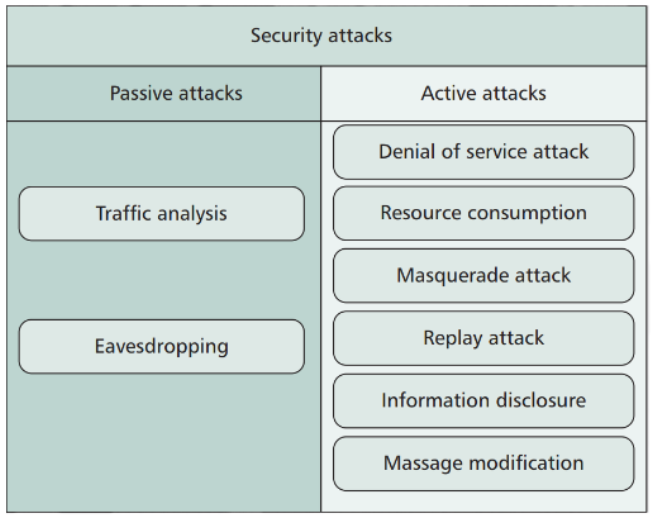
\includegraphics[width=0.5\textwidth]{img/wireless/attack classification.png}
    \caption{Active and passive attacks}
    \label{fig:active_passive_attacks}
\end{figure}
We are going to go through some of the most common attacks in wireless communication.
\begin{section}{Jamming}
   \begin{boxH}
     Jamming is a simple strategy to disrupt wireless communication by interfering with the
     communication channel.
    \end{boxH}
    It is usually carried out by broadcasting an interfering signal on a broad spectrum of frequencies
    to block the communication.\\
    A persistent and powerful adversary can always jam all data transmissions by transmitting 
    high-power white noise over the entire frequency spectrum.
    Jammer can be classified into two categories:
    \begin{itemize}
      \item \textbf{Active jamming}: the attacker continuously transmits a jamming signal to 
        interfere with the communication.
      \item \textbf{Reactive jamming}: the attacker only transmits a jamming signal when it
        detects a signal from the legitimate transmitter.
    \end{itemize}
    Although jamming is a difficult to address availability issue, it can be addressed via many
    physical layer security techniques.
    \end{section}
    \begin{section}{Eavesdropping}
      The wireless communication channel is a broadcast medium by nature. Because of this its 
      hard to eliminate unauthorized access to the wireless channel.\\
      To address those problesm, the most common way is to encrypt the data before transmitting it.\\
      Another widely used approach is to force the transmitter and receiver to adopt some 
      information hiding measures, by embedding private messages into a background signal or 
      noise process. In other words, we bury the information in the noise.\\
      Eavesdropping too can be addressed via physical layer security techniques.
\end{section}

\begin{section}{Physical Layer Security}
  In traditional systems, reliability is guaranteed by channel coding at the physical layer, while 
  security is ensured by encryption protocols at the upper layers, although in some cases we would 
  like to have security at the physical layer.\\
  This is possible because the physical layer has some unique properties that can be exploited to
  provide security, nominally the randomness of the wireless channel, which is an unpredictable
  and time-varying medium.\\

  \begin{boxH}
    \textbf{Physical layer security} aims at \textbf{exploiting the randomness} inherent in noisy channels to provide
    an additional level of protection at the physical layer.
  \end{boxH}
  
  \begin{figure}[h]
    \centering
    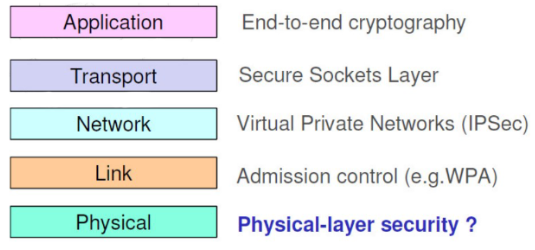
\includegraphics[width=0.5\textwidth]{img/wireless/layer security.png}
    \caption{Security measures at different layers}
    \label{fig:layer_security}
  \end{figure}
  A desirable proprety of the communication channel is \textbf{perfect secrecy}, which for a 
  wireless communication channel means that the channel is unknown to unauthorized users, or the 
  channel of the unauthorized users is more noisy than that of the authorized users.\\
  This means that we have a "better" channel than the eavesdropper, and we can obtain a that in 
  a different ways. For instance the sender and the receiver can cooperate, for example by choosing
  the same channel estimation method.\\

  In any case, security at physical layer is not intended to replace cryptographic security, but rather, it
  affords an additional protection layer. In fact, Physical Layer Security does not even allow 
  demodulation, which cryptographic security does.\\
  Nowadays, many results from information theory, signal processing, and cryptography
  suggest that there is much security to be gained by accounting for the imperfections of the
  physical layer when designing secure systems.

  Furthermore, physical layer security methods can be categorized into:
  \begin{itemize}
    \item \textbf{channel approaches}: such as fingerprinting, precoding and applying MIMO techniques.
    \item \textbf{code approaches}: adding cryptografy to error correction codes and applying spreading
      codes to the signal.
    \item \textbf{power approaches}: using direction antennas to make the communication less broad 
      or generating artificial noise to confuse the eavesdropper.
    \item \textbf{signal design approaches}: using artificial noise to degrade eavesdropper's 
      channel estimation
  \end{itemize}

  Each method addresses specific aspects of physical layer security, ranging from utilizing
  channel characteristics to employing artificial noise and directional antennas, and each one 
  is effective against different types of attacks.
  \begin{figure}[H]
    \centering
    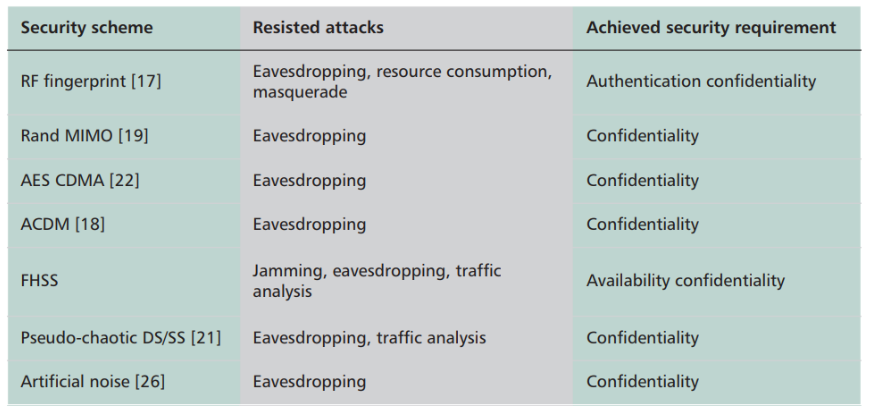
\includegraphics[width=0.8\textwidth]{img/wireless/physical layer security schema.png}
    \caption{Physical layer security methods}
    \label{fig:physical_layer_security_schema}
  \end{figure}

\end{section}

